\chapter{Introduction and Background Research}

% Introduction
% Related Works
    % Evaluation

% Join spectrums into one section

% You can cite chapters by using '\ref{chapter1}', where the label must
% match that given in the 'label' command, as on the next line.
\label{chapter1}

% Sections and sub-sections can be declared using \section and \subsection.
% There is also a \subsubsection, but consider carefully if you really need
% so many layers of section structure.
\section{Introduction}

%<A brief introduction suitable for a non-specialist, {\em i.e.} without using technical terms or jargon, as far as possible. This may be similar/the same as that in the 'Outline and Plan' document. The remainder of this chapter will normally cover everything to be assessed under the `Background Research` criterion in the mark scheme.>

Ocean surface simulation \ref{fig:ocean_simulation} is a field of computer graphics that aims to create realistic representations of the ocean surface.
It is an important area of research as it has a wide range of applications, including video games, movies.
In video games it used for inteactivity and visual apeal, while in movies it is used for visual apeal. 

There are many techniques that have been developed to simulate ocean surfaces, from the simple and fast algorithms as 
sum of sines or gersner waves to more complex techniques such as particle simulations and Fast Fourier Transform (FFT) Ocean \ref{fig:ocean_simulation}.

The primary objective of this project is to simulate a realistic ocean surface, 
one that does not exhibit any tiling or repeating patterns, and that can accurately 
represent stormy weather conditions. Therefore, using sum of sines or gerstner waves is not sufficient.

This is achieved by leveraging the power of the Inverse Fourier Transform (IFFT), a mathematical technique that transforms data 
from the frequency domain back to the time (or spatial) domain. In the context of this project, 
it allows us to transform the frequency data of the ocean waves into a spatial representation, i.e., the height map of the ocean surface. This is
desireble as it allows us to simulate realistic ocean surfaces that are not only visually appealing, but also physically accurate as 
we are using real-world data to generate frequencies.

\begin{minipage}{1\textwidth}
    \centering
    \includegraphics[width=0.75\textwidth]{"images/final_ocean_simulation.png"}
    \captionof{figure}{FFT Ocean Simulation}
    \label{fig:ocean_simulation}
\end{minipage}

\section{Gerstner Waves}
Gerstner waves provide a simple model for generating somewhat realistic ocean waves. This model is straightforward to implement and is predominantly used in video games. Even major titles, such as “Pokemon Legends: Arceus”, utilize something similar to Gerstner waves to simulate oceanic environments.
The concept of Gerstner waves was first introduced by F.J. Gerstner \cite{Franz1809} in 1802. The initial known implementation of Gerstner waves in computer graphics was carried out by Fournier and Reeves \cite{AlainWilliam1986} in 1986. The model is an attempt to approximate the motion of ocean waves, based on the principle that each point in the ocean undergoes a circular motion.
If a point is represented as $\mathbf{x_0} = (x_0, z_0)$, the height and horizontal displacements can be calculated as follows:
\begin{equation}
\mathbf{x} = \mathbf{x_0} - (\mathbf{k} / k) A \sin(\mathbf{k} \cdot \mathbf{x_0} - \omega t)
\end{equation}
\begin{equation}
    y = A \cos(\mathbf{k} \cdot \mathbf{x_0} - \omega t)
\end{equation}
\begin{equation}
    \omega = \sqrt{gk}
\end{equation}
Here, $A$ is the amplitude, $\omega$ is dispertion relationship, and $\mathbf{k}$ is a wave vector that points horizontally in the direction of wave travel and is proportional to the wavelength $\lambda$ of the wave.
\begin{equation}
k = 2 \pi / \lambda
\end{equation}
As presented, the Gerstner waves model is limited to a single wave. To simulate more complex ocean surfaces, multiple waves need to be summed together. This is achieved by summing the waves as follows:
\begin{equation}
\mathbf{x} = \mathbf{x_0} - \sum_{i=1}^{N} (\mathbf{k_i} / k_i) A_i \sin(\mathbf{k_i} \cdot \mathbf{x_0} - \omega_i t)
\end{equation}
Here, $N$ is the number of waves, $A_i$ is the set of amplitudes, $\omega_i$ is the set of frequencies, and $\mathbf{k}_i$ is the set of wave vectors.
The primary challenge with this approach is that simulating realistic ocean surfaces requires summing a large number of waves together, which can be computationally expensive. 
Furthermore, Gerstner waves offer limited artistic control, has visible tiling \ref{fig:pokemon_water_tiling}, and underperforms in simulating stormy weather conditions.

\begin{minipage}{1\textwidth}
    \centering
    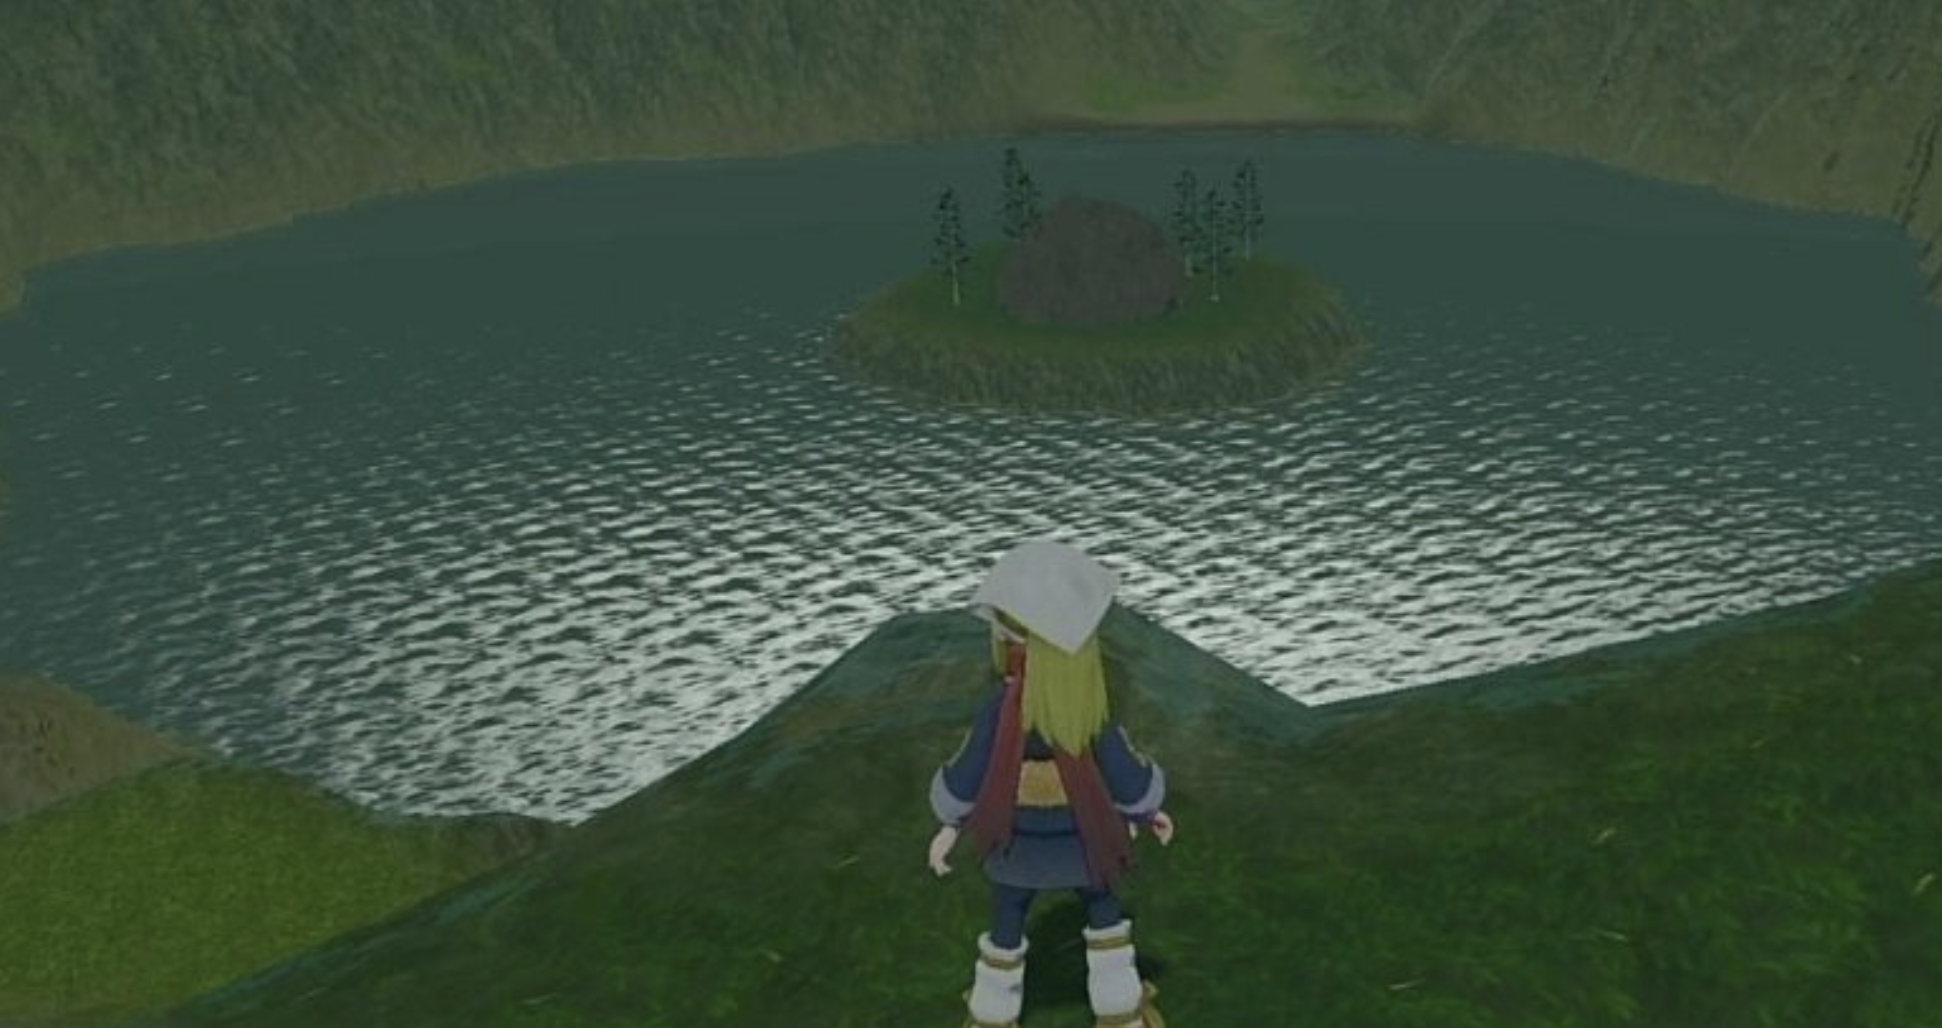
\includegraphics[width=0.75\textwidth]{"images/pokemon_water_tiling.png"}
    \captionof{figure}{Water Tiling in Pokemon Legends: Arceus}
    \label{fig:pokemon_water_tiling}
\end{minipage}

\section{Particle Simulation and Machine Learning}
Particle-based methods are commonly used for realistic water simulation, but they’re computationally expensive.
Recent advancements in Graphics Processing Unit (GPU) technology, coupled with innovative research such as that conducted by Libo Huang \cite{huang2021}, are progressively rendering particle simulations more feasible for ocean simulation. Nonetheless, these techniques necessitate a high-performance GPU and are not yet suitable for widespread real-time applications.

Furthermore, there have been significant strides in the application of machine learning to expedite fluid simulations, as evidenced by the work of Dmitrii Kochkov \cite{kochkov2021machine}. These methodologies, however, are exceedingly complex, necessitating expertise in both computer graphics and machine learning. Additionally, they require substantial volumes of data for model training.
Therefore, they will not be considered for this project.

\section{Fourier Transform}
The Fourier Transform is a mathematical method that enables us to convert our data from the time domain to the frequency domain, and vice versa. To simplify, imagine we have a smoothie that’s too sour. With the Fourier Transform, we could deconstruct our smoothie (time domain) into its ingredients (frequency domain), remove the sour component, and then reconstruct it back.
It was invented by Joseph Fourier\cite{fourier1822} in 1822, altough at his time it didn't have much practical use, however, nowdays it is used in many fields, including signal processing, image processing, and in our case ocean simulation.

To convert our data from the time domain to the frequency domain, we use the Fourier Transform:
\begin{equation}
\tilde{f}(\omega) = \int_{-\infty}^{\infty} f(x) e^{-i \omega x} dx
\end{equation}
, where $f(x)$ is the function in the time domain, $\tilde{f}(\omega)$ is the function in the frequency domain, and $\omega$ is a frequency.
To convert our data from the frequency domain back to the time domain, we use the Inverse Fourier Transform:
\begin{equation}
f(x) = \int_{-\infty}^{\infty} \tilde{f}(\omega) e^{i \omega x} d\omega
\end{equation}
As, we going to work with discrete data, we are going to use the Discrete Fourier Transform (DFT):
\begin{equation}
    x_n = \sum_{k=0}^{N-1} \tilde{x}_k e^{-i 2 \pi k n / N}
\end{equation}
and the Inverse Discrete Fourier Transform (IDFT):
\begin{equation}
    \tilde{x}_k = \frac{1}{N} \sum_{n=0}^{N-1} x_n e^{i 2 \pi k n / N}
    \label{eq:idft}
\end{equation}

\section{Fourier Transform Ocean}
The challenge with Gerstner waves is that we need to generate multiple waves for each vertex to simulate an ocean. This can be computationally expensive as an ocean can have thousands of vertices. To address this problem, J. Tessendorf\cite{tessendorf2001} proposed a method to generate ocean waves using the Fourier Transform.

The main idea is to generate a height map of the ocean surface in the frequency domain, and then convert it back to the time domain using the IFT. Since the IFT produces a periodic height map, we can tile it to create an infinite ocean surface. This means that we can generate one texture and apply it to the entire water body.

The advantage of this method becomes apparent when considering a 512x512 texture, which combines 262,144 distinct waves. In contrast, Gerstner waves experience noticeable performance loss after 65 waves.

To produce the height map, we first need a function that approximates the frequencies. We call this function a spectrum. J. Tessendorf uses a modified Phillips spectrum that generates Fourier amplitudes in the frequency domain:
\begin{equation}
    \tilde{h}_0(\mathbf{k}) = \frac{1}{\sqrt{2}}(\xi_r + \xi_i)\sqrt{P_h(\mathbf{k})}
    \label{eq:fouier_amplitudes}
\end{equation}
where $\xi_r$ and $\xi_i$ is complex number made from real and imaginary part that was drawn from a gaussian random number generator, with mean 0 and stardart deviation 1.

We then combine $\tilde{h}_0(\mathbf{k})$ with its conjugate $\tilde{h}^{*}_0(-\mathbf{k})$, to "produce waves towards and against the wave direction when propagating"\cite{horvath2015}:
\begin{equation}
    \tilde{h}(\mathbf{k}, t) = \tilde{h}_0(\mathbf{k})e^{i\omega(k)t}+\tilde{h}^{*}_0(-\mathbf{k})e^{-i\omega(k)t}
    \label{eq:combined_amplitudes}
\end{equation}

By performing the Inverse Discrete Fourier Transform (IDFT):
\begin{equation}
    h(\mathbf{x}) = \sum_{\mathbf{k}} \tilde{h}(\mathbf{k}, t)e^{i\mathbf{k}\cdot\mathbf{x}}
    \label{eq:height_map}
\end{equation}
we obtain the height map, where $\mathbf{x}=(x,y)$ is the position in the texture.

\begin{minipage}{1\textwidth}
    \centering
    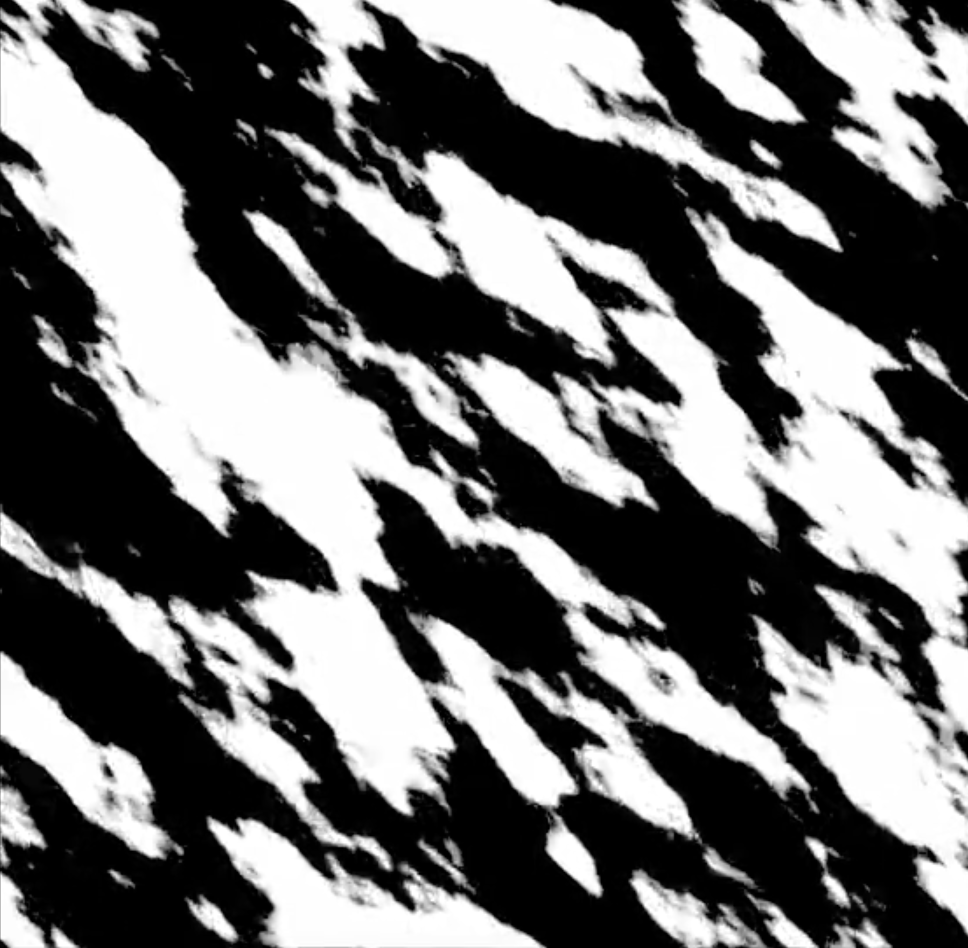
\includegraphics[width=0.4\textwidth]{"images/philips_height_map.png"}
    \captionof{figure}{Height Map using J. Tessendorf's Spectrum}
\end{minipage}

\section{Ocean Spectrums}
\subsection{Jerry Tessendorf's Ocean Spectrum}
The main thing that defines how ocean will looks is the spectrum. Inside Jerry Tessendorf's \cite{tessendorf2001} paper, he proposed modified Phillips spectrum \ref{fig:phillips_spectrum}:
\begin{equation}
    P_h(\mathbf{k}) = A \frac{e^{-1/(kL)^{2}}}{k^{4}}| \mathbf{\hat{k}} \cdot \mathbf{w} |^{6}
    \label{eq:tessendorf_spectrum}
\end{equation}
where $A$ is numeric constant, $L = V^2/g$ is the largest possible wave arising from wind speed $V$ and gravity $g$. The $| \mathbf{\hat{k}} \cdot \mathbf{w} |^{6}$ is used to surpress waves that are moving perpendicular to the wind direction.
However, J. Tessendorf admits that this spectrum has "poor convergence properties at high values of the wavenumber $|\mathbf{k}|$ and suggests to surpress waves that are $l \leq L$, where $l$ is some small constant and multiply the Phillips spectrum by $e^{-k^2l^2}$.

\subsection{JONSWAP Spectrum}
Regarding all the issues that we experiance with "Phillips Spectrum", Horvath Christopher \cite{horvath2015} proposed to use JONSWAP spectrum.
JONSWAP stands for "Joint North Sea Wave Project" and was developed by Hasselmann \cite[et al. in 1973]{hasselmann1973}. This spectrum is improved version of Pierson-Moskowitz Spectrum \cite{pierson1964} when Horvath noticed that the wave spectrum is never fully developed.
Therefore he added extra peak enchancement factor $\gamma^r$.\\
The JONSWAP spectrum is defined as follows:
\begin{equation}
    \begin{aligned}
        S_{\text{JONSWAP}}(\omega) &= \frac{\alpha g^{2}}{\omega^{5}} \exp \left(-\frac{5}{4} \left(\frac{\omega_{p}}{\omega}\right)^{4}\right) \gamma^{r} \\
        &r = \exp\left(-\frac{(\omega - \omega_p)^{2}}{2 \sigma^{2}\omega^{2}_p}\right) \\
        &\alpha = 0.076 \left( \frac{U^{2}_{10}}{Fg} \right)^{0.22} \\
        &\omega_p = 22 \left( \frac{g^{2}}{U_{10}F} \right)^{1/3} \\
        &\gamma = 3.3 \\
        &\sigma = 
        \begin{cases} 
        0.07 & \text{if } \omega \leq \omega_p \\
        0.09 & \text{if } \omega > \omega_p
        \end{cases}
    \end{aligned}
\end{equation}

where F is the fetch (distance to lee shore), $U_{10}$ is the wind speed at 10 meters above the sea level and $\omega$ is angular frequency.

\subsection{The Texel MARSEN ARSLOE (TMA) Spectrum}
The biggest problem with with JONSWAP spectrum is that it only works with deep waters. Therefore, Horvath Christopher \cite{horvath2015} proposed to use TMA correction for deep water spectrum.
TMA was developed by Steven A. Hughes \cite{hughes1984}, based on the observations made by Kitaigordskii \cite{kitaigordskii1975}.
this is known as Kitaigordskii depth Attenuation function and it takes form:
\begin{equation}
    \begin{aligned}
        \Phi(\omega_h) &= \left[ \frac{(k(\omega, k))^{-3}\frac{\partial k(\omega, h)}{\partial \omega}}{(k(\omega, \infty ))^{-3}\frac{\partial k(\omega, \infty)}{\partial \omega}} \right] \\
        \omega_h &= \omega \sqrt{h/g}
    \end{aligned}
\end{equation}
where h is the depth of the water. At first glance this function seems to be difficult, however looking at \ref{fig:tma_correction} we can see that this can be easilly approximated.

\begin{minipage}{1\textwidth}
    \centering
    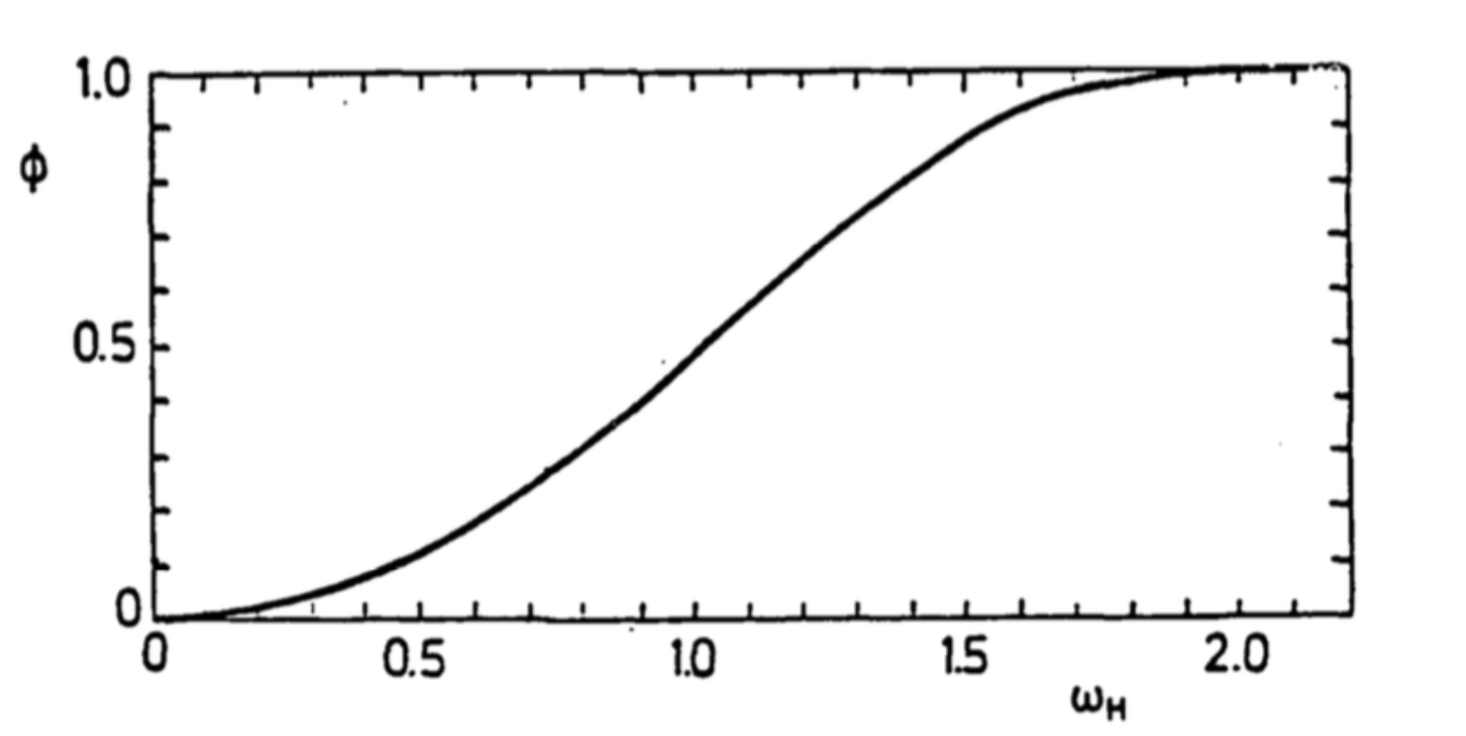
\includegraphics[width=0.65\textwidth]{"images/tma_correction.png"}
    \captionof{figure}{$\Phi(\omega, h)$ as a function of $\omega_h$ \cite{hughes1984}}
    \label{fig:tma_correction}
\end{minipage}

Approximation given by Thomson and Vincent \cite{thompson1983} is:
\begin{equation}
    \begin{aligned}
        &\Phi(\omega, h) \approx
        \begin{cases} 
        \frac{1}{2} \omega_h^{2} & \text{if } \omega_h \leq 1 \\
        1 - \frac{1}{2}(2 - \omega_h)^{2} & \text{if } \omega_h > 1
        \end{cases}
    \end{aligned}
\end{equation}

With $\Phi(\omega, h)$ we can now correct the JONSWAP spectrum for shallow waters:
\begin{equation}
    S_{\text{TMA}}(\omega, h) = S_{\text{JONSWAP}}(\omega) \Phi(\omega, h)
    \label{eq:tma_spectrum}
\end{equation}

\subsubsection{Donelan-Banner Directional Spreading}
Currentlly we can't use the TMA sprectrum for our project as it has few problems. Firstlly, this spectrum is non-directional, so we need to add directionality to it. Secondly, this spectrum accepts $\omega$ as input, but as we following J. Tessendorf's \cite{tessendorf2001} paper, we need to use $\mathbf{k}$ as input.
To solve this problem Horvath Christopher \cite{horvath2015} proposes to use Donelan-Banner Directional Spreading \cite{young1999}:
\begin{equation}
    D(\omega, \theta) = \frac{\beta_s}{2 \tanh(\beta_s\pi)}\text{sech}(\beta_s\theta)^{2}
\end{equation}
where,
$$
\begin{aligned}
    &\beta_s =
    \begin{cases} 
    2.61(\omega/\omega_p)^{1.3} & \text{for } 0.56 < \omega/\omega_p < 0.95 \\
    2.28(\omega/\omega_p)^{-1.3} & \text{for } 0.95 \leq \omega/\omega_p < 1.6 \\
    10^{\epsilon} & \text{for } \omega/\omega_p \geq 1.6
    \end{cases}
\end{aligned}
$$
$$
\epsilon = -0.4 + 0.8393 \cdot e^{-0.567\ln(\omega/\omega_p)^{2}}
$$
$$
\theta = \arctan(k.y / k.x) - \theta_{\text{wind}}
$$

In our project we will use $\omega/\omega_p < 0.95$ for first case as it produces more smooth results.
Now we can combine the TMA spectrum with the Donelan-Banner Directional Spreading:
\begin{equation}
    D_{\text{TMA}}(\omega, \theta) = S_{\text{TMA}}(\omega) \cdot D(\omega, \theta)
\end{equation}

\subsubsection{TMA transformation}
Lastlly, to make this spectrum usable we need to transform it from $\omega$ to $\mathbf{k}$ and according to Horvath Christopher \cite{horvath2015} we can transform it like this:
\begin{equation}
    S_{\text{TMA}}(\mathbf{k}) = 2S_{\text{TMA}}(\omega, h) \cdot \frac{d\omega}{dk} / k \cdot \Delta k_x \cdot \Delta k_y
    \label{eq:tma_spectrum_k}
\end{equation}
where in our case,
$$
\frac{d\omega}{dk} = \frac{g}{2\sqrt{g*\mathbf{k}}}
$$

\section{Cooley-Tukey Fast Fourier Transform (FFT)}
When simulating fourier transform ocean majority times is spent on converting from frequency domain to time domain, in other words performing Inverse Fourier Transform.
Earlier mentioned IDFT \ref{eq:idft} has time complexity of $O(n^2)$, and it's clearlly that this algorithm is not sufficient to simulate heiger resolution ocean surfaces in real time.
In 1805 Gauss Carl Friedrich \cite{gauss1866} invented FFT algorithm $O(n\log n)$ and in 1965 Cooley James W. and Tukey John W. \cite{cooley1965} reinvented it.
The FFT algorithm is based on that there is redundancy in the computation of the DFT, and that we can exploit it to reduce the time complexity, it is important to mention that the FFT algorithm works only when the number of samples is a power of 2.

The basic idea of the FFT algorithm is as follows:
\begin{enumerate}
    \item Split the input data into two sets, one containing the even samples and the other containing the odd samples and repeat this proccess until a set has 2 samples (bit-reverse sort order).
    \item Generate twiddle factor $W_N = e^{-i 2 \pi k / N}$ and rise it to the power of \\
    \begin{equation}
        k = i * N / 2^{\text{stage} + 1} \text{ mod } N
    \end{equation}
    where $i$ is the index of the sample, stage is the current stage and $N$ is the number of samples.
    \item Perform butterfly operations \ref{fig:butterfly_diagram}, where $x$ and $y$ are complex numbers and $W$ is the twiddle factor
    \begin{minipage}{1\textwidth}
        \centering
        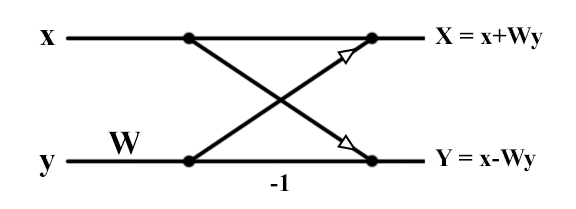
\includegraphics[width=0.5\textwidth]{"images/butterfly_diagram.png"}
        \captionof{figure}{Butterfly Diagram}
        \label{fig:butterfly_diagram}
    \end{minipage}
    \item The butterfly operations are performed in stages \ref{fig:8_butterfly_diagram}. For example, if we have 8 samples, we will have $\log(8) = 3 $ stages. The first stage is for pairs of points (2-point DFTs), the second stage is for groups of four points (4-point DFTs), and so on.
    \begin{minipage}{1\textwidth}
        \centering
        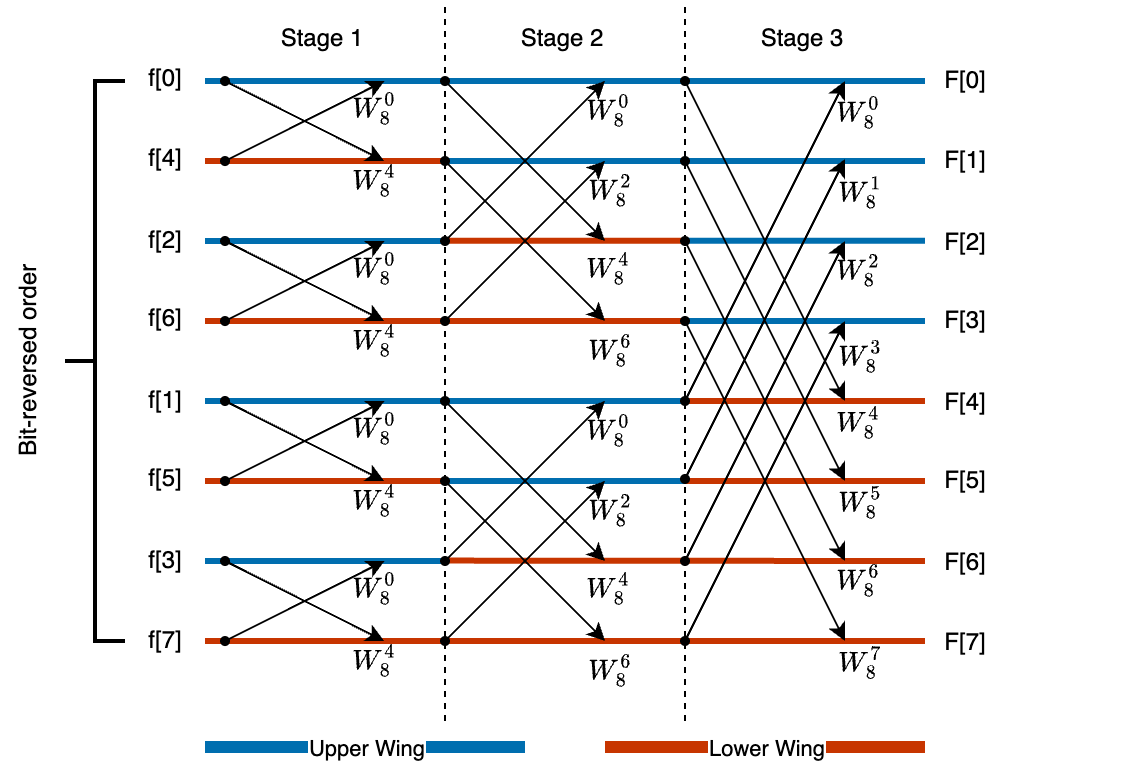
\includegraphics[width=0.7\textwidth]{"images/8_butterfly_diagram.png"}
        \captionof{figure}{8-point FFT Butterfly Diagram}
        \label{fig:8_butterfly_diagram}
    \end{minipage}
\end{enumerate}




% Introdunction on my project
% What is ocean simulation
% Why is it important
% What are the applications

% What other people are doing.
% Gersner waves
% FT Ocean
% Diffrent Spectrums
% FFT


% What I do is that is different from others.
% I combined this and this. From there and there.

% Why did I combine these papers and what do I suspect to get out.


